\documentclass{article}
\usepackage{graphicx} % Required for inserting images
\graphicspath{{./images/}}
\usepackage[utf8]{inputenc}
\usepackage{amsthm}
\usepackage{amsmath}
\usepackage{amssymb}
\usepackage{mathtools}
\usepackage{hyperref}
\usepackage[a4paper]{geometry}

\title{Caractérisation des singularités de type $\J$}
\author{Félix Larose-Gervais}
\date{Été 2023}

\newtheorem{definition}{Définition}
\newtheorem{proposition}{Proposition}
\newtheorem{conjecture}{Conjecture}
\newtheorem{example}{Exemple}
\newtheorem{corollary}{Corollaire}
\renewcommand*{\proofname}{Preuve}

\newcommand{\J}{\mathfrak{J}}
\newcommand{\JS}{\overline{\J}}

\begin{document}

\maketitle

\tableofcontents

\newpage

\section{Introduction}

\subsection{Notations}

Soit $a, b \in \mathbb{Z}$ on note la relation de coprimalité $\perp$

\[ a \perp b \iff \gcd(a, b) = 1 \]
Soit $m, n \in \mathbb{N}$, $X$ un ensemble, notons 

\begin{itemize}
    \item $S_m$ le groupe symmétrique à $m$ lettres
    \item $\mathbb{Z}_n$ l'anneau des entiers modulo n ($\mathbb{Z}/n\mathbb{Z}$)
    \item $\mathbb{Z}_n^\times$ son groupe d'inversibles ($\{ a \in \mathbb{Z}_n \mid a \perp n \})$
    \item $X^m$ l'ensemble des m-uplets de $X$ $(\underbrace{X \times \cdots \times X}_{m fois})$
\end{itemize}
On notera aussi $S_n^m$ l'ensemble des m-uplets d'inversibles modulo n $({({\mathbb{Z}_n^\times})}^m)$

\subsection{Définitions}

\begin{definition}
    Une \textbf{singularité} est un $[a] = ([a_1], \dots, [a_m]) \in S_n^m$, on appelle \begin{itemize}
        \item $n$ la \textbf{racine} de la singularité
        \item $[a_1], \dots, [a_m]$ les \textbf{poids} de la singularité
    \end{itemize}
\end{definition}

\begin{definition}
    Un \textbf{éclatement} $a \in \mathbb{Z}^m$ d'une singularité $[a] \in S_n^m$ (noté $a \in [a]$) est un choix de 
    représentant $a = (a_1, \dots, a_m)$ tel que
    \begin{align*}
        \forall i \neq j & : a_i \perp a_j
    \end{align*}
    On note $E_a$ l'ensemble des singularités associées à l'éclatement $a$ comme suit:
    \begin{align*}
        E_a & = \{ [a^i] \in S_{a_i}^m \mid \forall i = 1..m,\; a_i > 1 \} \\
        [a^i] & = ([a^i_1], \dots, [a^i_m]) \\
        [a^i_j] & \equiv \begin{cases}
            -n & \text{si $i = j$} \\
            a_j & \text{sinon}
        \end{cases} \pmod{a_i} \quad \forall j = 1..m
    \end{align*}
    On appelle $a = (a_1, \dots, a_m)$ \textbf{l'éclatement naturel} de $[a]$ si 
    les $a_1, \dots, a_m$ sont les plus petits représentant positifs de leurs classes
\end{definition}

\begin{definition}
    Un éclatement $a \in [a]$ est dit \textbf{lisse} si $a = (1, \dots, 1)$
\end{definition}

\begin{definition}
    La singularité $[a]$ est dite de \textbf{type $\J$} (noté $[a] \in \J$) ssi
    \begin{align*}
        \exists a \in [a] : E_a \subset \J
    \end{align*}
    On parlera de \textbf{type $\J$ strict} (noté $[a] \in \JS$) lorsque 
    pour $a \in [a]$ l'éclatement naturel de $[a]$ on a
    \begin{align*}
        E_a \subset \JS
    \end{align*}
\end{definition}

\newpage

\subsection{Rappels d'arithmétique}

\subsubsection{Algorithme d'Euclide et PGCD}

Soit $a, b \in \mathbb{Z}$, on calcule le PGCD comme suit
\begin{align*}
    \gcd(a, b) & := \begin{cases}
        a & \text{ si $b = 0$} \\
        \gcd(b, a \mod b) & \text{ sinon}
    \end{cases}
\end{align*}
Avec $k \in \mathbb{Z}$, on a les propriétés suivantes:
\begin{align*}
    \gcd(a, 1) & = 1 \\
    \gcd(a, b) & = \gcd(b, a) \\
    \gcd(a, b) &= \gcd(a, -b) \\
    \gcd(a, b) & = \gcd(a, b + ka)
\end{align*}
De la dernière on déduit directement, pour $n \in \mathbb{N}$
\begin{align*}
        a \equiv b \pmod n \implies \gcd(a, n) = \gcd(b, n)
\end{align*}

\subsubsection{Théorème des restes chinois}

Soit $m, n_1, \dots, n_m \in \mathbb{N}$ et $a_1, \dots, a_m \in \mathbb{Z}$, notons le produit $n = n_1 \cdots n_m$

Si $\forall i \neq j : n_i \perp n_j$, alors $\exists!x \in \mathbb{Z}_n$ tel que
\begin{align*}
    x &\equiv a_1 \pmod {n_1} \\
    &\vdotswithin{\equiv} \\
    x &\equiv a_m \pmod {n_m}
\end{align*}

\newpage

\subsection{Résultats connus}
Résultats utiles, dûs à Habib Jaber.

\begin{proposition}
    Soit $a, b \in \mathbb{Z}$
    \[ a \perp b \implies {(a, b)}_{a + b} \in \JS \]
\end{proposition}

\begin{example}
    $8 \perp 5 \implies {(8, 5)}_{13} \in \JS$
\end{example}
\begin{figure}[h]
    \caption{Illustration avec la suite de Fibonacci}
    \centering
    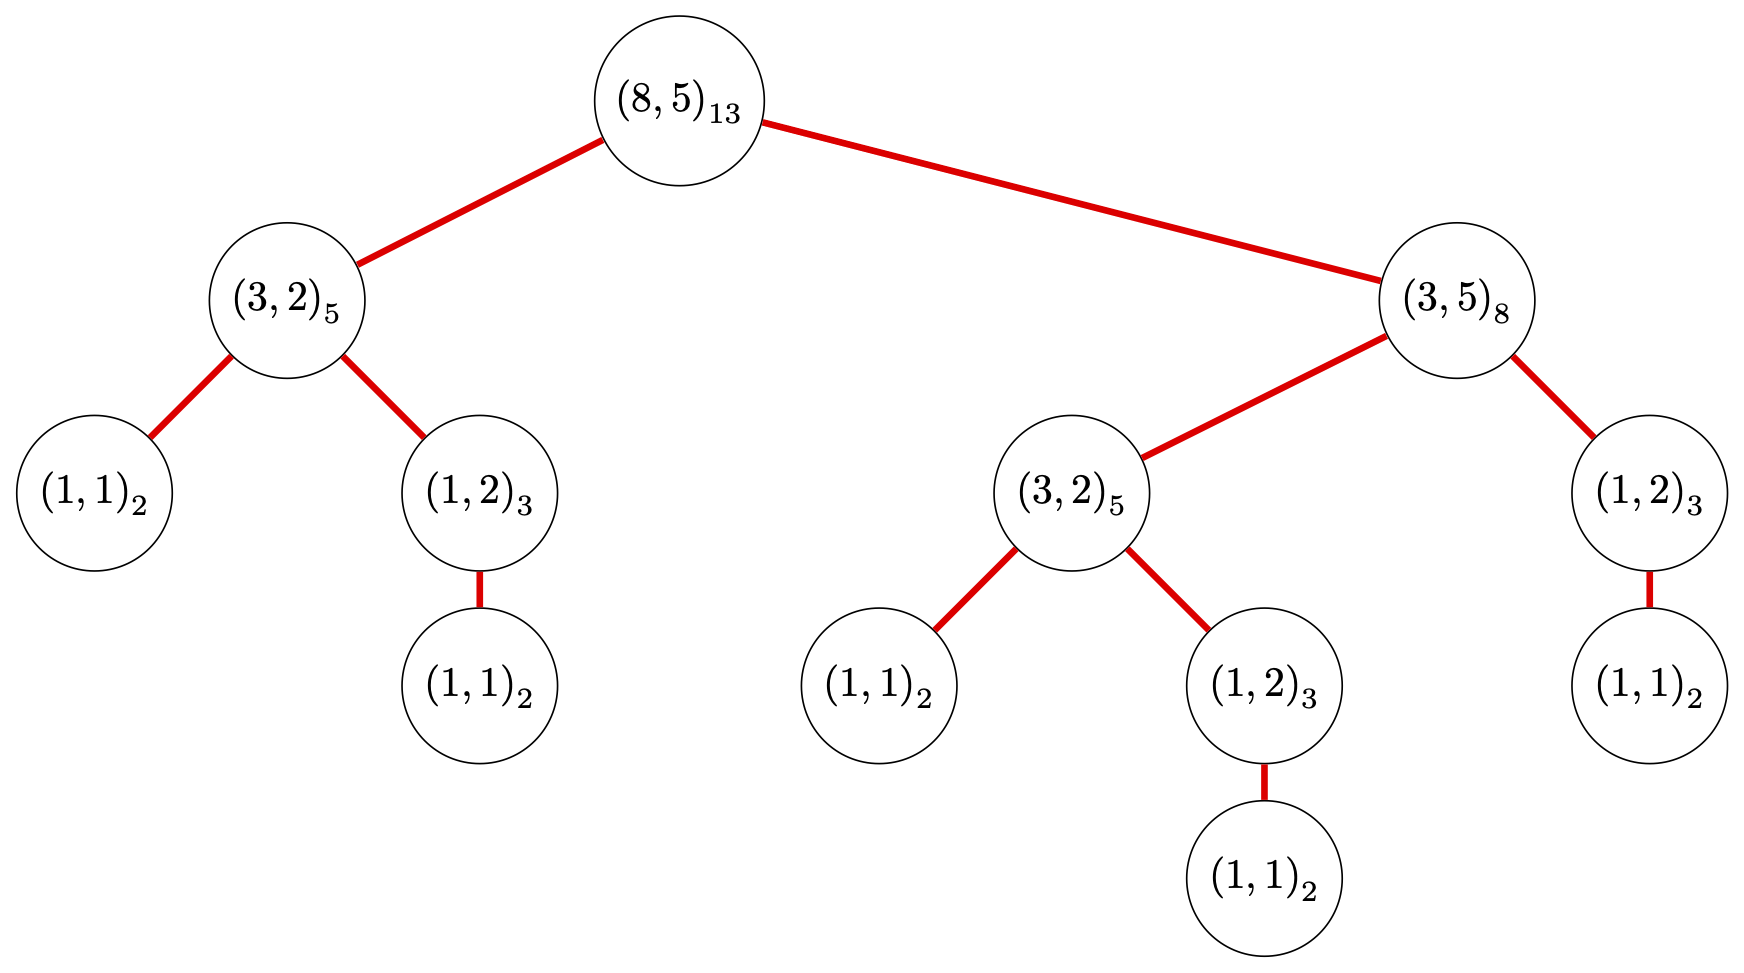
\includegraphics[width=0.8\textwidth]{fibo}
\end{figure}

\begin{proposition}
    Soit $a, b \in \mathbb{Z}$
    \[ {(a, b)}_n \in \JS \implies \forall k \in \mathbb{Z}^\times : {(a, b)}_{n+kab} \in \JS \]
\end{proposition}

\begin{example}
    ${[(3, 2)]}_5 \in \JS \implies {(3, 2)}_{11} \in \JS$
\end{example}

\begin{figure}[h]
    \caption{${(3, 2)}_5 \cong {(3, 2)}_{11}$}
    \centering
    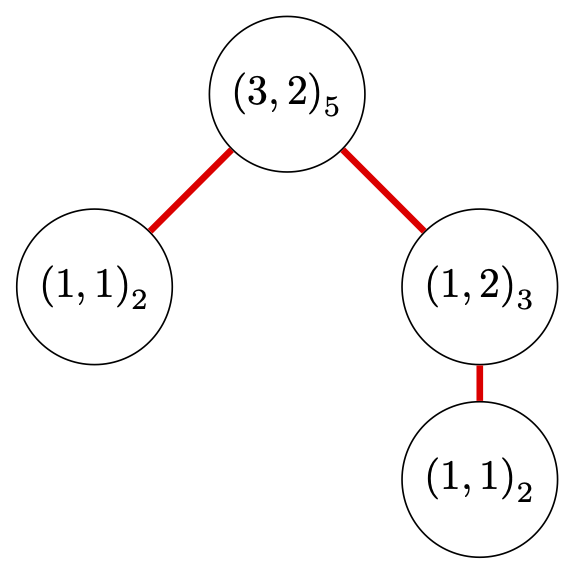
\includegraphics[width=0.3\textwidth]{532}
    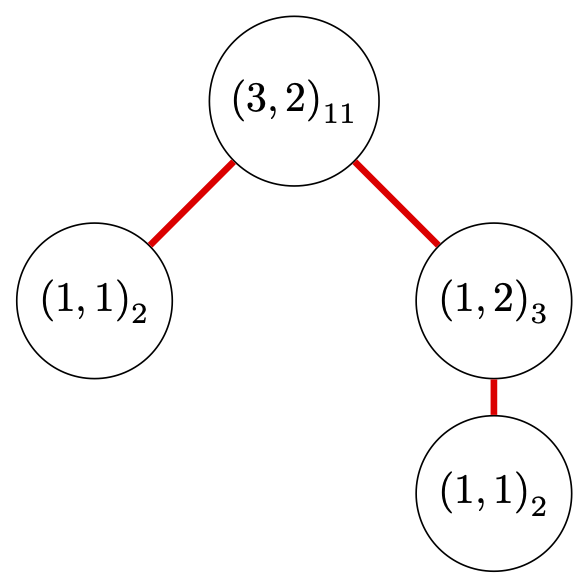
\includegraphics[width=0.3\textwidth]{11_3_2}
\end{figure}

\newpage

\section{Propositions}

Soit $m, n \in \mathbb{N}$ tels que $m, n \geq 2$ et une singularité $[a] = {([a_1], \dots, [a_m])}_n \in S_n^m$

\subsection{Existence d'un éclatement}

\begin{proposition}
    Toute singularité isolée admet un éclatement
\end{proposition}

\begin{proof}
    Prenons $(a_1, \dots, a_m) \in [a]$ le représentant naturel de $[a]$

    On cherche $(b_1, \dots, b_m) \in [a]$ tels que $\forall i \neq j : b_i \perp b_j$ et $\forall i : b_i \perp n$

    Il suffit de prendre $b_1 = a_1$ et $\forall i = 2..m$, un $b_i$ vérifiant
    \begin{align*}
        b_i & \equiv a_i \pmod n \\
        b_i & \equiv 1 \pmod {b_1} \\
            & \vdotswithin{\equiv} \\
        b_i & \equiv 1 \pmod {b_{i-1}}
    \end{align*}

    De tels $b_i$ existent par le théorème des restes chinois

    On vérifie les coprimalités nécéssaires grâce aux propriétés de $\gcd$
    
    \hspace{\parindent} On a par la première congruence $\forall i : b_i \perp n$ (puisque $\forall i : a_i \perp n$)

    \hspace{\parindent} Et par les suivantes $\forall i \neq j : b_i \perp b_j$

    On a donc $b = (b_1, \dots, b_m)$ un éclatement de $[a]$
\end{proof}

\subsection{Propriétés}

\subsubsection{Symmétrie}

\begin{proposition}
    Le réarrangement des poids préserve le type $\J$. Soit $\sigma \in S_m$, on a
    \[ [a] \in \J \implies \sigma([a]) \in \J \]
\end{proposition}

\begin{proof}
    Prenons $a \in [a]$ tel que $E_a \subset \J$

    Il suffit d'observer que $E_a \cong E_{\sigma(a)}$
\end{proof}

\begin{figure}[h]
    \caption{Illustration avec $a = (a_1, a_2)$, $\sigma = (12)$}
    \centering
    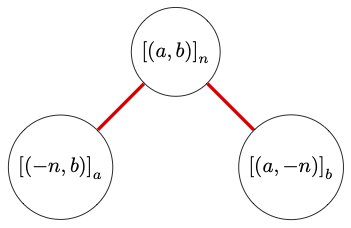
\includegraphics[width=0.4\textwidth]{abn}
    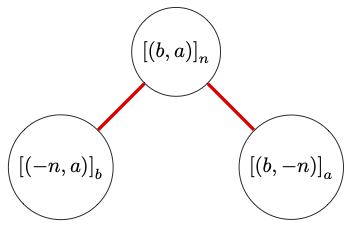
\includegraphics[width=0.4\textwidth]{ban}
\end{figure}

\subsubsection{Ajout de poids}

\begin{proposition}
    L'ajout de poids de valeur 1 préserve le type $\J$
    \[ {([a_1], \dots, [a_m])}_n \in \J \implies {([a_1], \dots, [a_m], [1])}_n \in \J \]
\end{proposition}

\begin{proof}
    Prenons $a \in [a]$ tel que $E_a \subset \J$, $b = (a_1, \dots, a_m, 1)$

    Il suffit d'observer que $E_a \cong E_b$
\end{proof}

\begin{figure}[h]
    \caption{Illustration avec $a = (a_1, a_2)$}
    \centering
    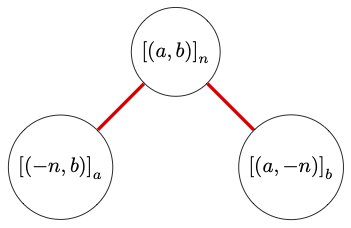
\includegraphics[width=0.4\textwidth]{abn}
    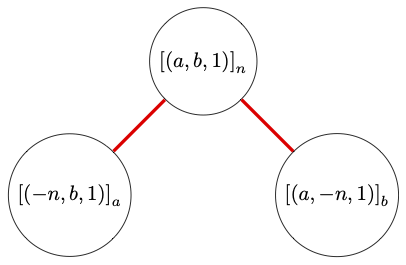
\includegraphics[width=0.4\textwidth]{ab1n}
\end{figure}

\subsubsection{Retrait de poids}

\begin{proposition}
    Le retrait de poids préserve le type $\J$
    \begin{align*}
        {([a_1], \dots, [a_m])}_n \in \J \implies {([a_1], \dots, [a_{m-1}])}_n \in \J
    \end{align*}
\end{proposition}

\begin{proof}
    Prenons $a \in [a]$ tel que $E_a \subset \J$

    La preuve se fait par induction structurelle

    D'abord, on observe ${([1], \dots, [1])}_n \in \J$

    Puis on suppose que $\forall [b] \in E_a : [b] \in \J \implies {([b_1], \dots, [b_{m-1}])}_n \in \J$

    On en conclut ${([a_1], \dots, [a_{m-1}])}_n \in \J$

\end{proof}

\begin{figure}[h]
    \caption{Illustration pour $m = 3$}
    \centering
    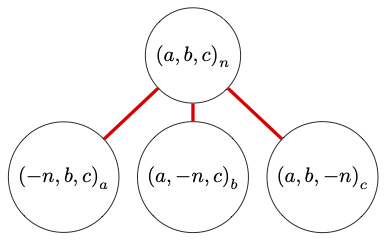
\includegraphics[width=0.4\textwidth]{abcn}
    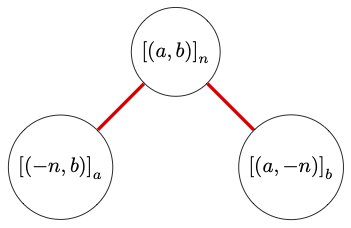
\includegraphics[width=0.4\textwidth]{abn}
\end{figure}

\newpage

\subsection{Caractérisation stricte}

\begin{proposition}
    Soit $[a] \in S_n^2$, d'éclatement naturel $a = (a_1, a_2) \in [a]$
    \[ [a] \in \JS \implies n \geq a_1 + a_2 \]
\end{proposition} 

\begin{proof}
    Par contraposée, supposons $n < a_1 + a_2$ ($\star$)

    \begin{itemize}
        \item Si $a_1 = a_2$ ($\neq 1$ par ($\star$))

            Alors $[a] \not \in \JS$
        \item Sinon, $a_1 \neq a_2$, supposons sans perdre de généralité que $a_1 > a_2$

            Considérons $a^1$ l'éclatement naturel de $[a^1] \in E_a$ la singularité associée à $a_1$

            On a $a^1 = (-n \mod a_1,\; a_2 \mod a_1)$

            \begin{itemize}
                \item Puisque $a_1 > a_2$, on a $2a_1 > a_1 + a_2 > n$, donc $a_1 < n < 2a_1$
                    
                On en déduit $(-n \mod a_1) = 2a_1 - n$

                \item Aussi, $(a_2 \mod a_1) = a_2$ car $a_1 > a_2$
            \end{itemize}

            On a donc $a^1 = (2a_1-n,\; a_2)$

            Puisque $n < a_1 + a_2$, on a $a_1 < 2a_1 - n + a_2$

            Donc $[a^1] \in S_{a_1}^2$ vérifie la condition ($\star$), on répète le raisonnement avec $[a^1]$
    \end{itemize}
\end{proof}

\begin{example}
    ${(4, 3)}_5 \not \in \JS$ car $5 < 4 + 3$
\end{example}

\begin{figure}[h]
    \caption{Singularités $s \in S_{32}^2$ telles que $s \in \JS$}
    \centering
    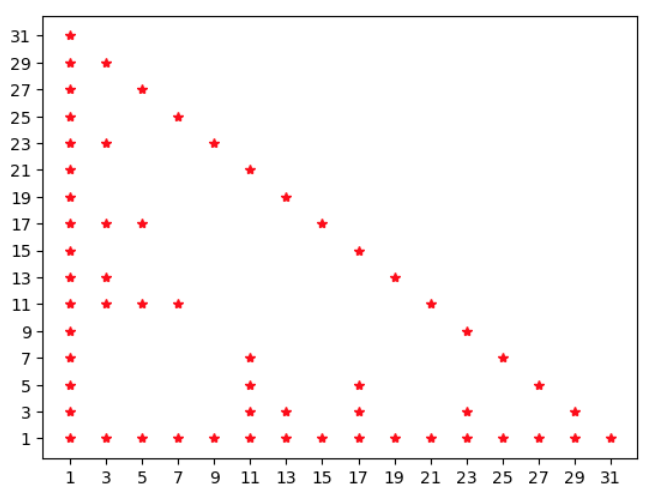
\includegraphics[width=0.7\textwidth]{singularite_j_strict_m2_n32}
\end{figure}

\newpage

\section{Conjectures}

\begin{conjecture}
    Soit $[a] \in S_n^m$ de représentant naturel $a = (a_1, \dots, a_m) \in \mathbb{Z}^m$
    \begin{align*}
        [a] \in \JS \implies |E_a| \leq 2
    \end{align*}
\end{conjecture}

\begin{proof}
    Supposons par contraposée $|E_a| > 2$ ($\star$)

    Donc, sans perdre de généralité, on a $a_1 > a_2 > a_3 > 1$

    On a donc les singularités $[a^1], [a^2] \in E_a$ d'éclatements naturels $a^1, a^2$

    $\cdots$ donc avec $a > b > c > 1$ copremiers deux-à-deux

    ${(b, c)}_a \in \JS$ et ${(a_b, c)}_b \in \JS$ contradiction?
\end{proof}

\begin{figure}[h]
    \caption{Singularités $s \in S_{13}^3$ telles que $s \in \JS$}
    \centering
    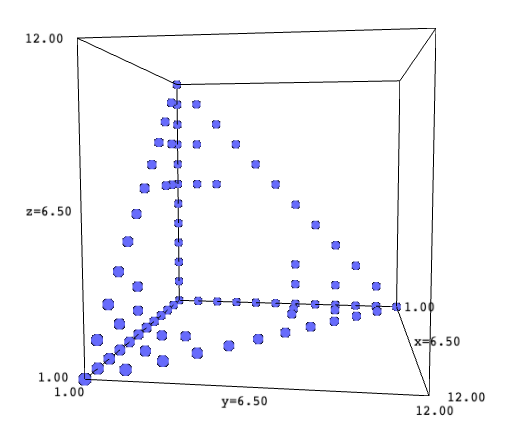
\includegraphics[width=0.6\textwidth]{singularite_j_strict_m3_n13}
\end{figure}

\begin{corollary}
    Soit la singularite $[a] \in S_n^m$ de représentant naturel $a = (a_1, a_2, \dots, a_m) \in \mathbb{Z}^m$

    Supposons sans perdre de généralité que $a_1 > a_2 > \cdots > a_m$, alors
    \begin{align*}
        [a] \in \JS \iff a_3 = \cdots = a_m = 1 \text{ et } {[(a_1, a_2)]}_n \in \JS
    \end{align*}
\end{corollary}

\begin{proof} D'après les proposition précédentes
    \begin{itemize}
        \item ($\impliedby$) Si $a_3 = \cdots = a_m = 1 \text{ et } {[(a_1, a_2)]}_n \in \JS$
        
            Comme ${[(a_1, a_2)]}_n \in \JS$, on a $[a] \in \JS$ (par ajout de poids à 1)
        \item ($\implies$) Si $[a] \in \JS$

            Alors $a = (a_1, a_2, 1, \dots, 1)$  (par la conjecture)

            Et $[(a_1, a_2)] \in \JS$ (par retrait de poids)
    \end{itemize}
\end{proof}

\newpage

\begin{conjecture} (Antisymmétrie) Soit $a > 1$, alors
    \[ {(a, b)}_n \in \JS \implies {(-a, b)}_n \not \in \JS \]
\end{conjecture}

\begin{corollary}
    Soit $a > 1$, alors
    \[ {(a, b)}_n \in \JS \implies {(n, b)}_a \not \in \JS \]
\end{corollary}

\begin{proof}
    Si ${(a, b)}_n \in \JS$, alors son éclatement ${(-n, b)}_a \in \JS$ (car $a > 1$)

    Par la conjecture précédente, ${(n, b)}_a \not \in \JS$
\end{proof}

\begin{corollary}
    Soit $n > a > b > c > 1$, alors
    \[ {[(a, b, c)]}_n \not \in \JS \]
\end{corollary}

\begin{conjecture}
    Si $[a] \in \JS$, alors $[a] \in \J$, donc $\J = \JS$
\end{conjecture}


\end{document}
